\documentclass[11pt]{article}

\usepackage{multicol}
%\usepackage{mwe}
\usepackage{subfigure}
\usepackage{mathtools}
\usepackage{graphicx}
\usepackage{amsmath}
\usepackage{mathrsfs}
\usepackage[top=0.5in,bottom=1in,left=1in,right=1in]{geometry}
\usepackage{pdflscape}
\usepackage{times}
\usepackage{bm}
%\usepackage{setspace}
\usepackage{color}
\usepackage{caption}
\usepackage{amsmath}
\usepackage{amssymb}
%\usepackage{CJK}
\usepackage{longtable}
%\usepackage[final]{pdfpages}
\usepackage{listings}
\usepackage{textcomp}
\usepackage{xcolor}
\usepackage{algorithm2e}
\usepackage{float}
\usepackage{algorithmicx}
\usepackage{algpseudocode}
\usepackage{hyperref}

\hypersetup{hidelinks,
	colorlinks=true,
	allcolors=black,
	pdfstartview=Fit,
	breaklinks=true}

\pagestyle{plain}




\begin{document}

\title{report on implementation models}
\author{SXY,SYF}
\date{\today}

\maketitle % need full-width title

\section{Abstract}

This document compares three models: the AM94 model (a rewarded or non-rewarded $\epsilon$ 
model situated between a null model and an AM model), the AM model (a modified 
two-stage $\epsilon$ model), and the SR model (a two-stage arbitration model). All convergence 
results are based on the convergence of states (2,1) and states (2,2), using the 
parameter values {$\alpha = 0.25, \beta = 0.0005, \delta = 0.25, convergence_time = 500, 
and max_iteration = 100000$}. These parameter settings align with those in AEU papers, 
even though they might not be optimal. Nonetheless, we can still gain insights into the 
mechanisms through simulations.

We run 10 sessions and take average of the results


\section{experiments of AM94, AM, SR implementation model}

\subsection{AM94 with reward}
Rewarded AM94 models can be compared with SR model for $\epsilon = 1$
\subsubsection{AM94 with reward on $\epsilon = 0.5$}

\begin{figure}[H]
	\begin{center}
	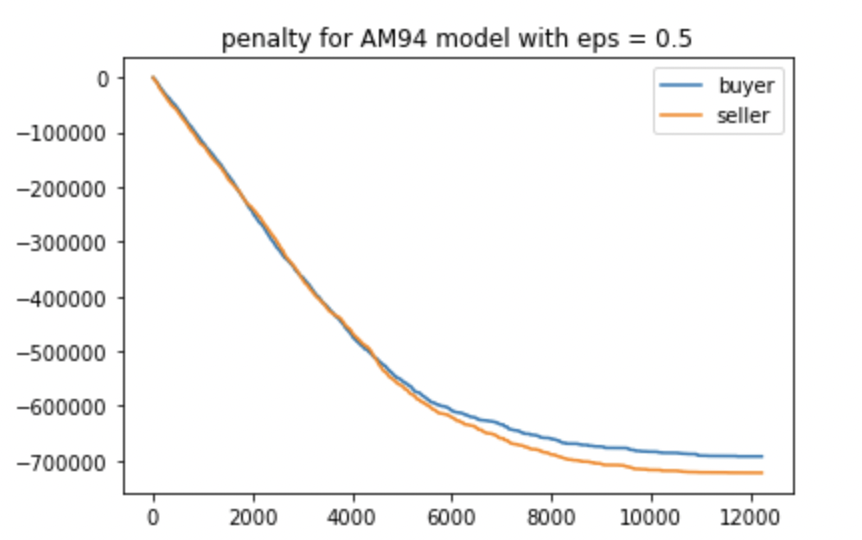
\includegraphics[width=0.9\textwidth]{1.PNG}
	\end{center}
	\caption{full penalty,with reward}
	\label{FIG.1}
\end{figure}

\begin{figure}[H]
	\begin{center}
	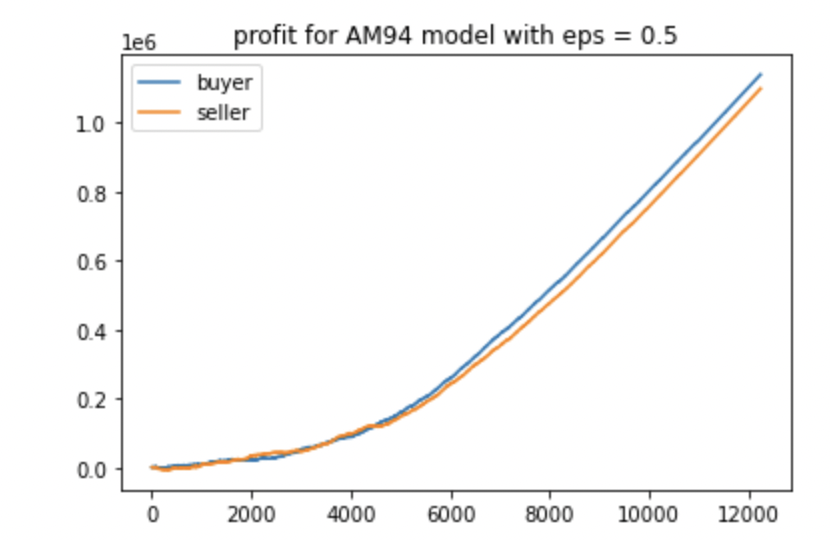
\includegraphics[width=0.9\textwidth]{2.PNG}
	\end{center}
	\caption{full profit,with reward}
	\label{FIG.2}
\end{figure}

\begin{figure}[H]
	\begin{center}
	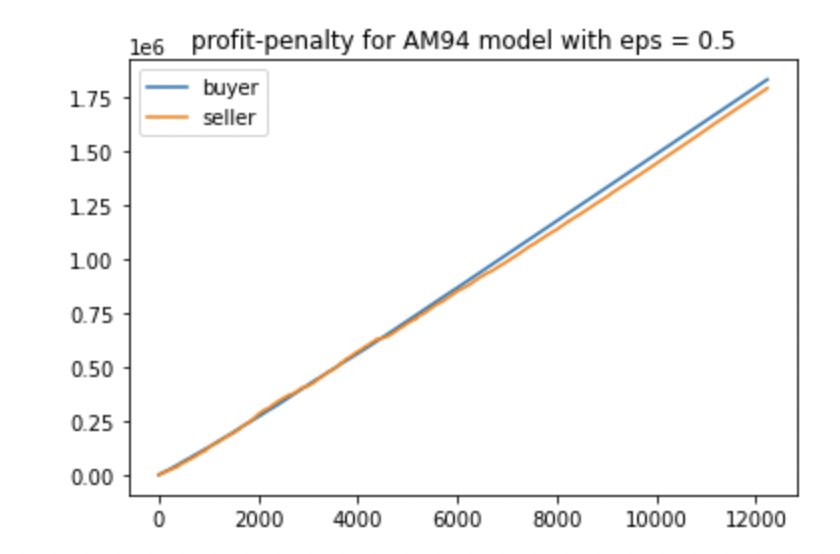
\includegraphics[width=0.9\textwidth]{3.PNG}
	\end{center}
	\caption{profit - penalty,with reward}
	\label{FIG.3}
\end{figure}	

If we consider only successful implementation situations, we can get other 3 pictures

\begin{figure}[H]
	\begin{center}
	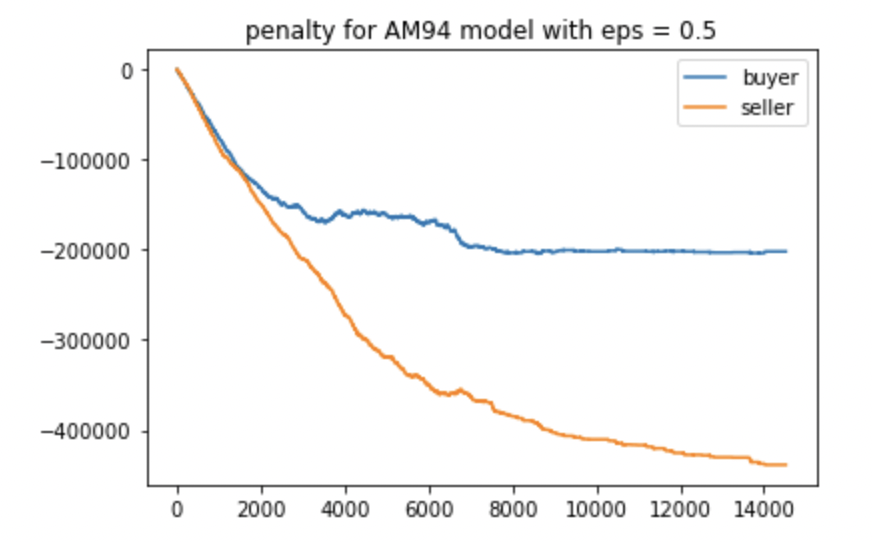
\includegraphics[width=0.9\textwidth]{4.PNG}
	\end{center}
	\caption{full penalty,with reward,implementation}
	\label{FIG.4}
\end{figure}

\begin{figure}[H]
	\begin{center}
	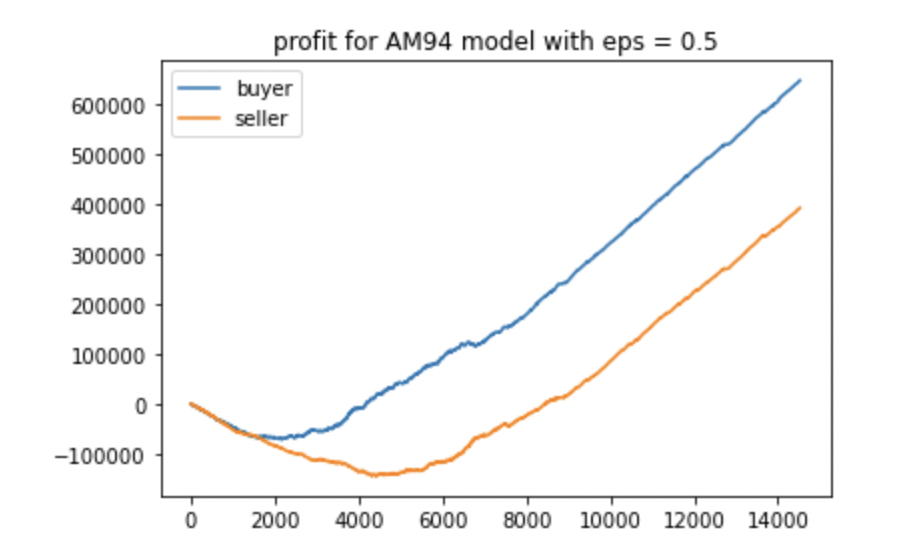
\includegraphics[width=0.9\textwidth]{5.PNG}
	\end{center}
	\caption{full profit,with reward,implementation}
	\label{FIG.5}
\end{figure}

\begin{figure}[H]
	\begin{center}
	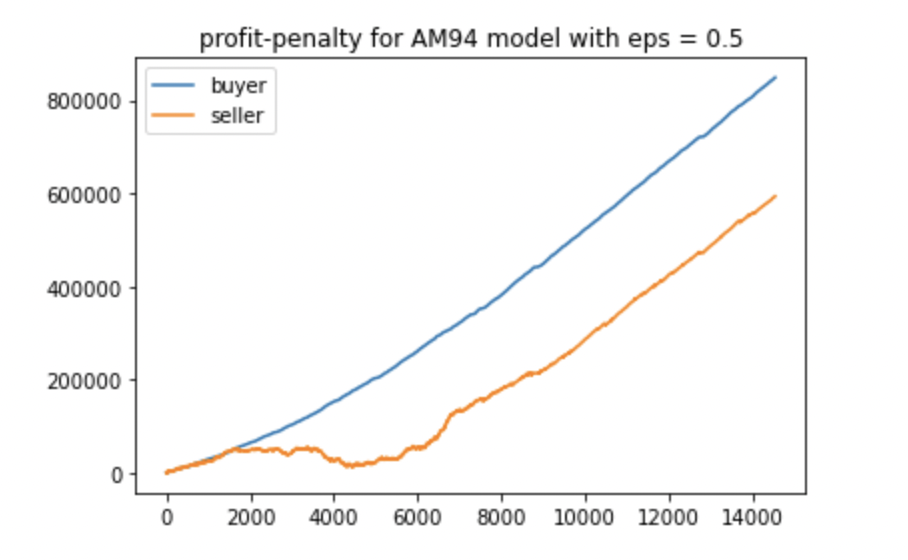
\includegraphics[width=0.9\textwidth]{6.PNG}
	\end{center}
	\caption{profit - penalty,with reward,implementation}
	\label{FIG.6}
\end{figure}

\subsubsection{AM94 with reward on $\epsilon = 0.4$}

\begin{figure}[H]
	\begin{center}
	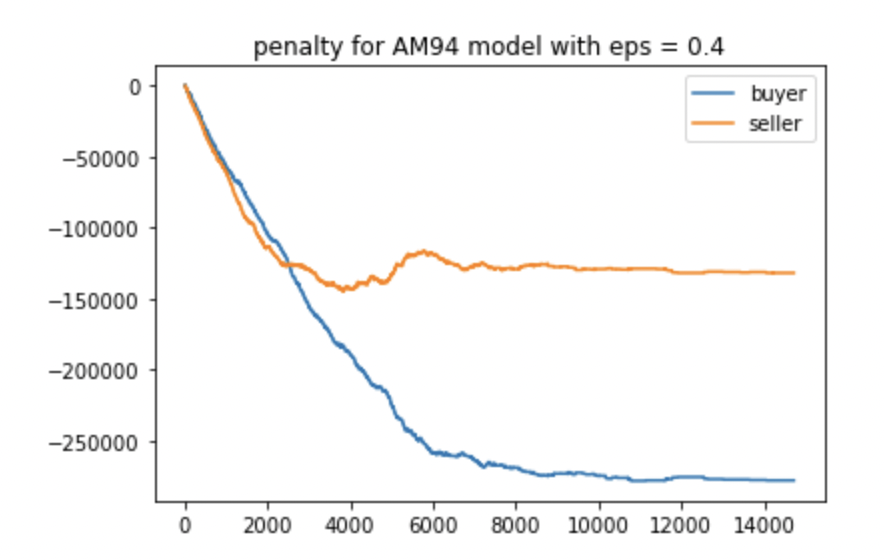
\includegraphics[width=0.9\textwidth]{7.PNG}
	\end{center}
	\caption{full penalty,with reward}
	\label{FIG.7}
\end{figure}

\begin{figure}[H]
	\begin{center}
	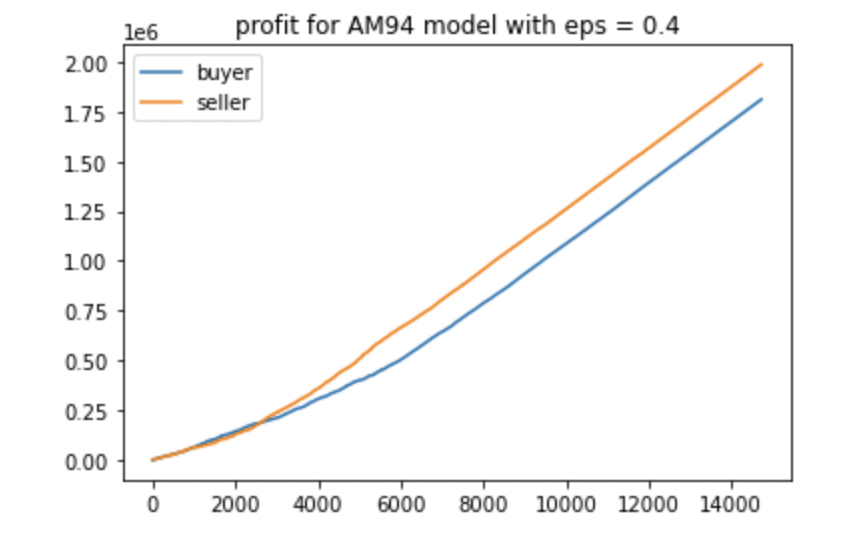
\includegraphics[width=0.9\textwidth]{8.PNG}
	\end{center}
	\caption{full profit,with reward}
	\label{FIG.8}
\end{figure}

\begin{figure}[H]
	\begin{center}
	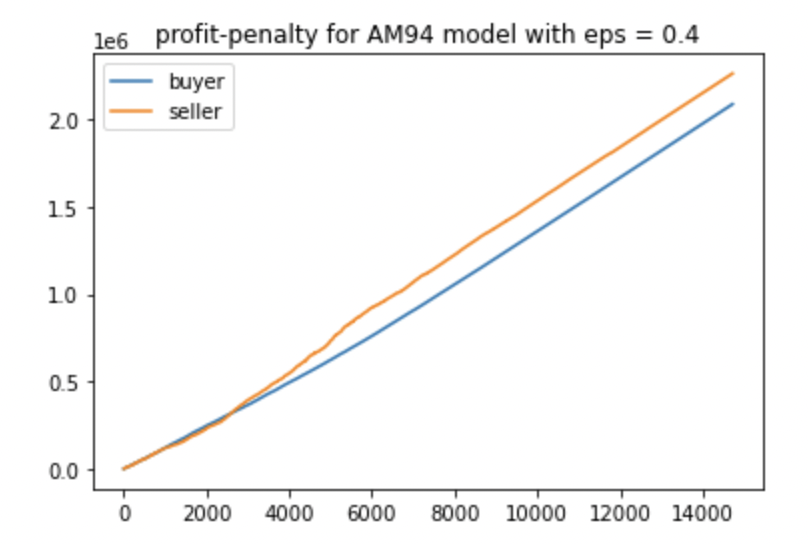
\includegraphics[width=0.9\textwidth]{9.PNG}
	\end{center}
	\caption{profit - penalty,with reward}
	\label{FIG.9}
\end{figure}	

If we consider only successful implementation situations, we can get other 3 pictures

\begin{figure}[H]
	\begin{center}
	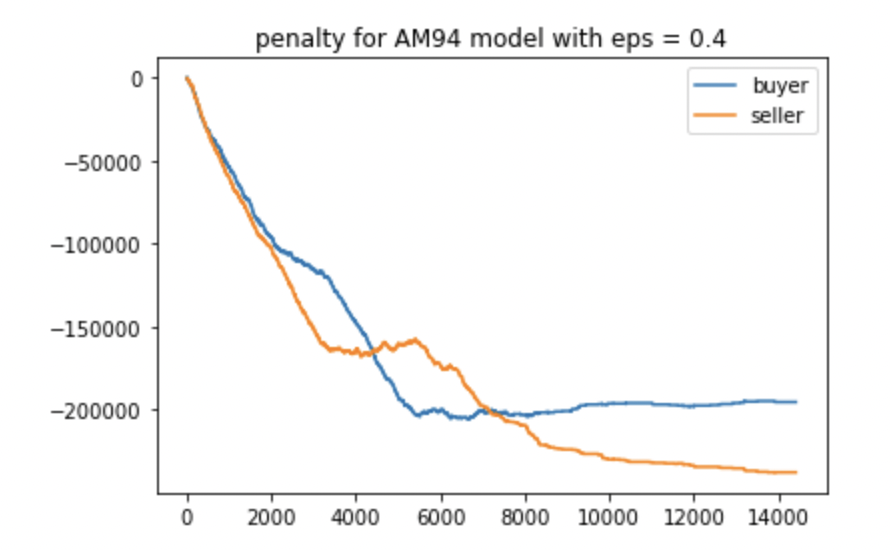
\includegraphics[width=0.9\textwidth]{10.PNG}
	\end{center}
	\caption{full penalty,with reward,implementation}
	\label{FIG.10}
\end{figure}

\begin{figure}[H]
	\begin{center}
	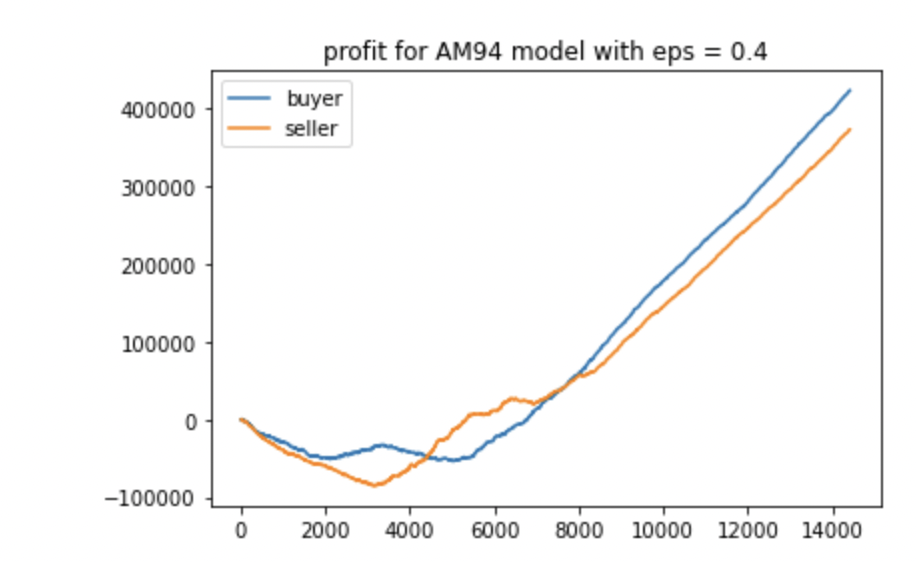
\includegraphics[width=0.9\textwidth]{11.PNG}
	\end{center}
	\caption{full profit,with reward,implementation}
	\label{FIG.11}
\end{figure}

\begin{figure}[H]
	\begin{center}
	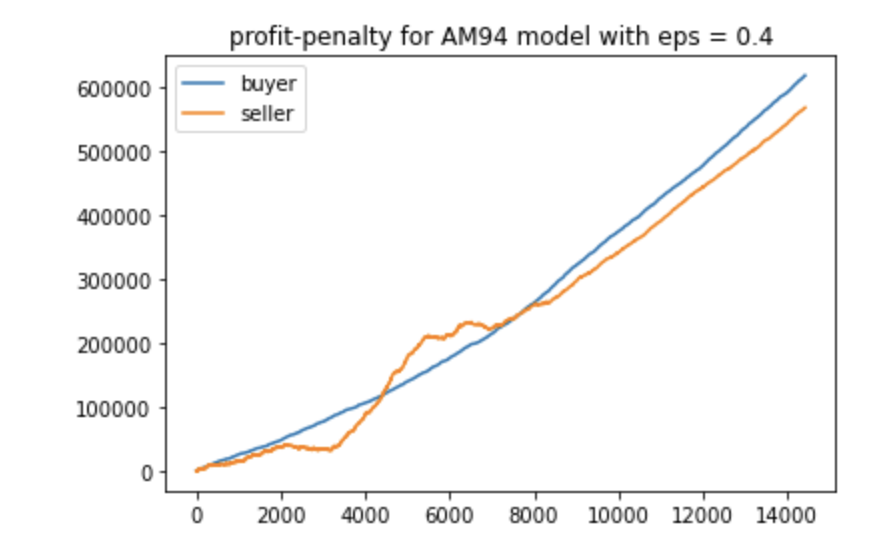
\includegraphics[width=0.9\textwidth]{12.PNG}
	\end{center}
	\caption{profit - penalty,with reward,implementation}
	\label{FIG.12}
\end{figure}


\subsubsection{AM94 with reward on $\epsilon = 0.3$}
the turning point is around 0.33, so this result does not converge.

\begin{figure}[H]
	\begin{center}
	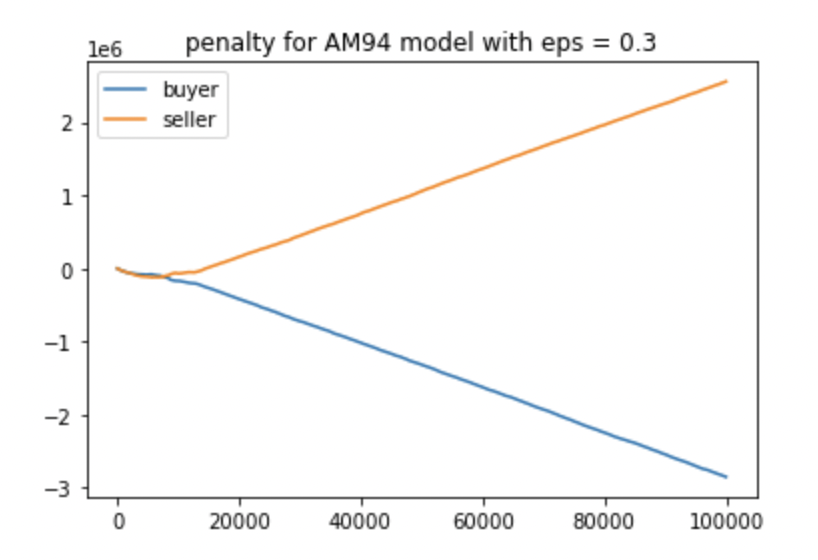
\includegraphics[width=0.9\textwidth]{13.PNG}
	\end{center}
	\caption{full penalty,with reward}
	\label{FIG.13}
\end{figure}

\begin{figure}[H]
	\begin{center}
	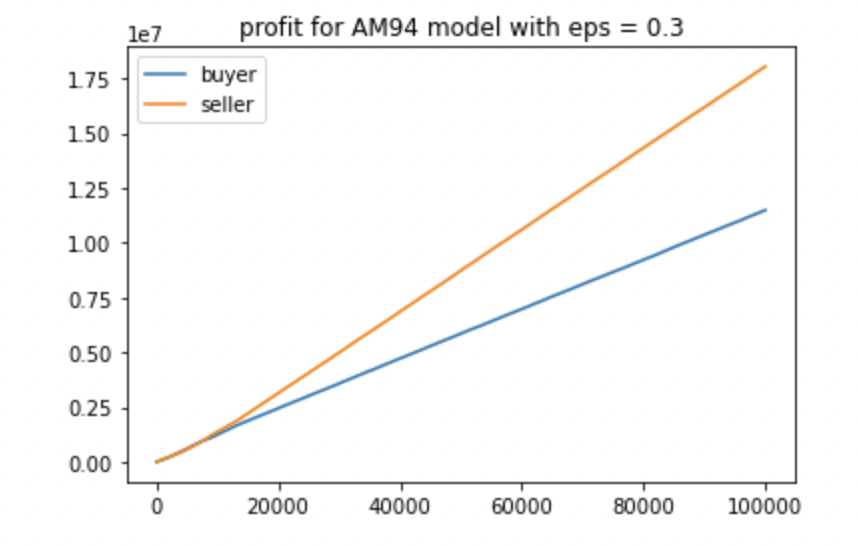
\includegraphics[width=0.9\textwidth]{14.PNG}
	\end{center}
	\caption{full profit,with reward}
	\label{FIG.14}
\end{figure}

\begin{figure}[H]
	\begin{center}
	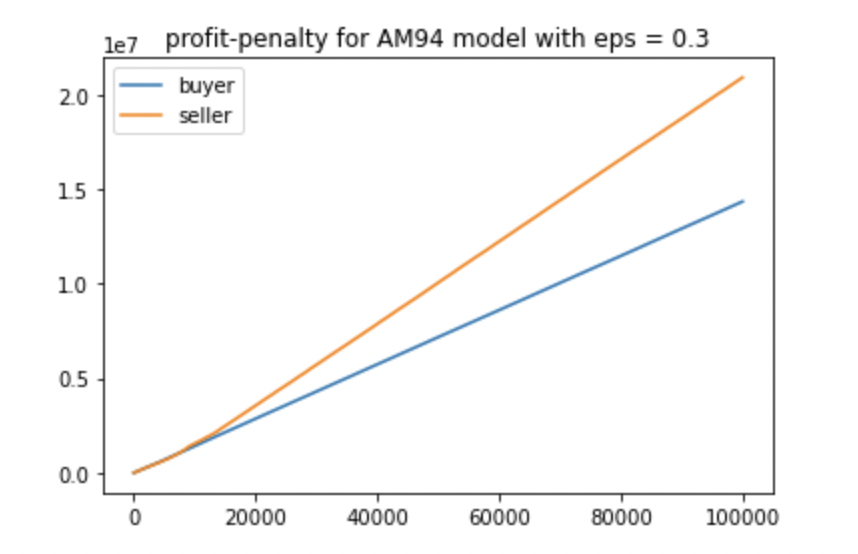
\includegraphics[width=0.9\textwidth]{15.PNG}
	\end{center}
	\caption{profit - penalty,with reward}
	\label{FIG.15}
\end{figure}	

If we consider only successful implementation situations, we can get other 3 pictures

\begin{figure}[H]
	\begin{center}
	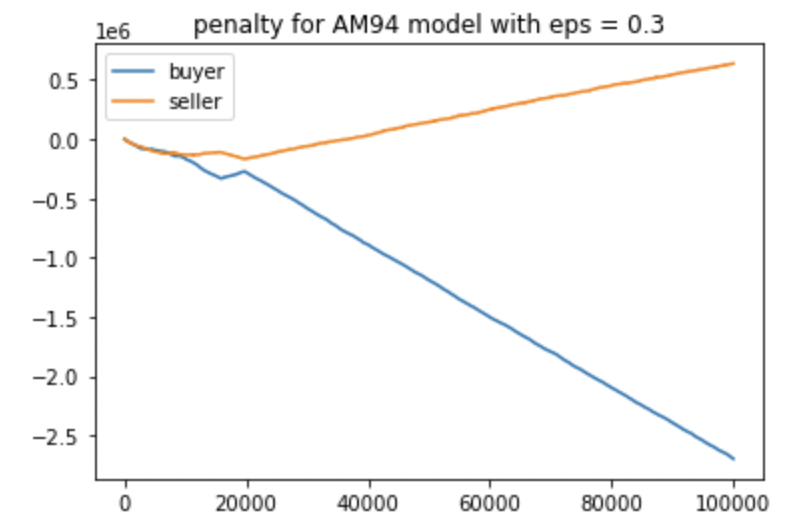
\includegraphics[width=0.9\textwidth]{16.PNG}
	\end{center}
	\caption{full penalty,with reward,implementation}
	\label{FIG.16}
\end{figure}

\begin{figure}[H]
	\begin{center}
	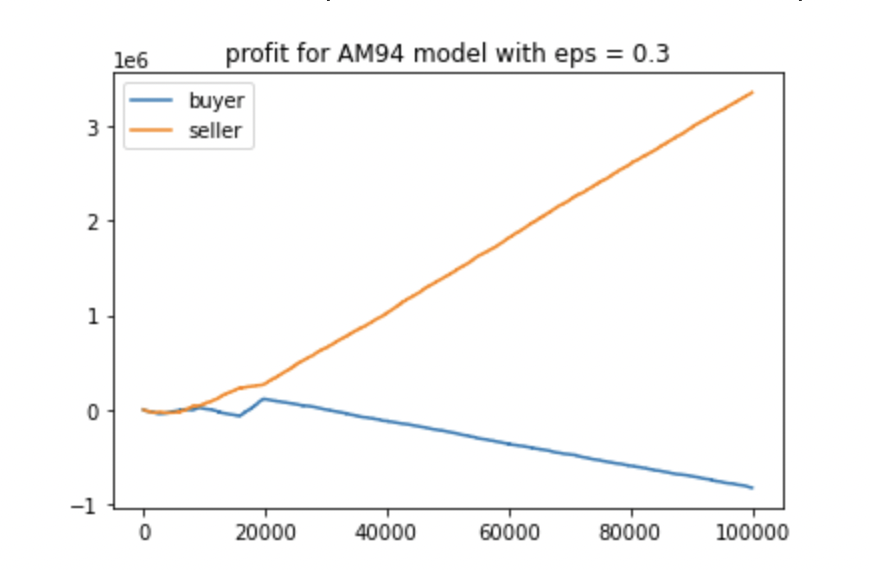
\includegraphics[width=0.9\textwidth]{17.PNG}
	\end{center}
	\caption{full profit,with reward,implementation}
	\label{FIG.17}
\end{figure}

\begin{figure}[H]
	\begin{center}
	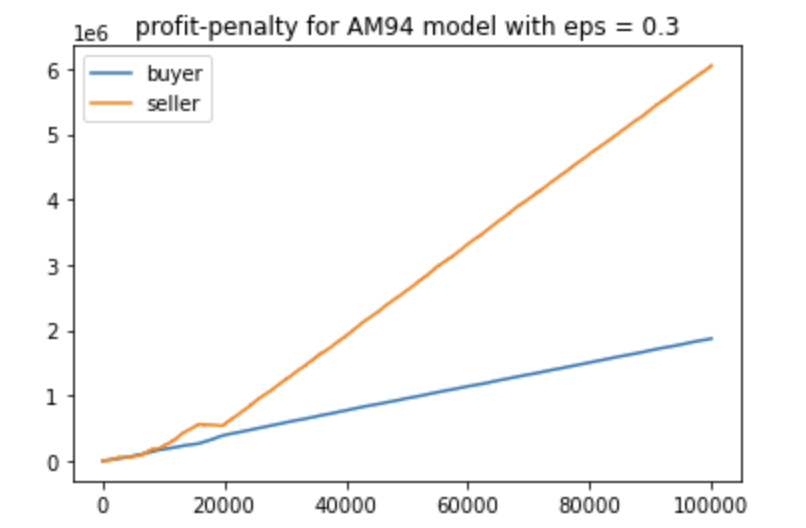
\includegraphics[width=0.9\textwidth]{18.PNG}
	\end{center}
	\caption{profit - penalty,with reward,implementation}
	\label{FIG.18}
\end{figure}


\subsection{AM94 with no reward}
Non Rewarded AM94 models can be compared with AM model for $\epsilon = 1$
\subsubsection{AM94 with no reward on $\epsilon = 0.5$}

\begin{figure}[H]
	\begin{center}
	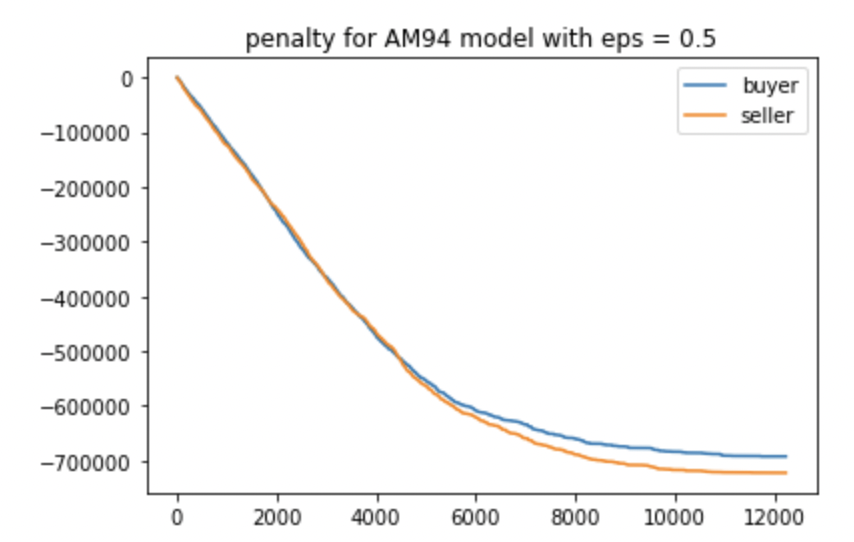
\includegraphics[width=0.9\textwidth]{19.PNG}
	\end{center}
	\caption{full penalty,no reward}
	\label{FIG.19}
\end{figure}

\begin{figure}[H]
	\begin{center}
	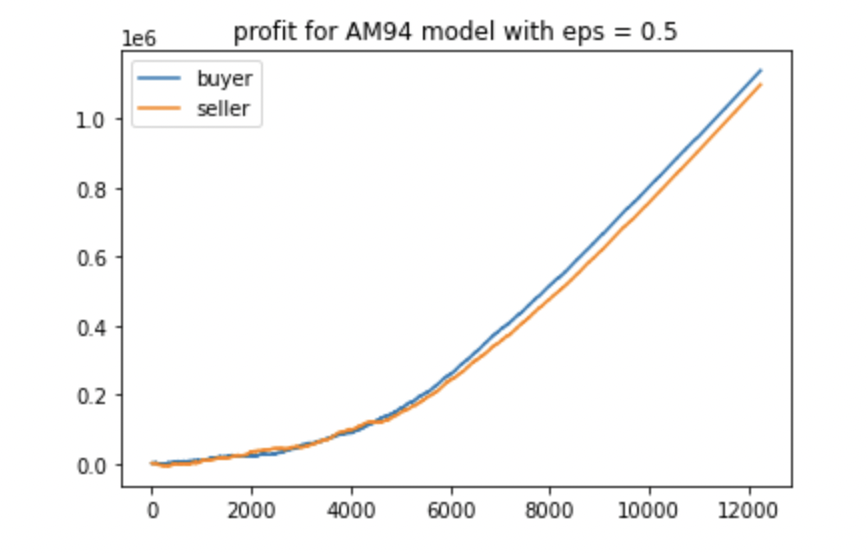
\includegraphics[width=0.9\textwidth]{20.PNG}
	\end{center}
	\caption{full profit,no reward}
	\label{FIG.20}
\end{figure}

\begin{figure}[H]
	\begin{center}
	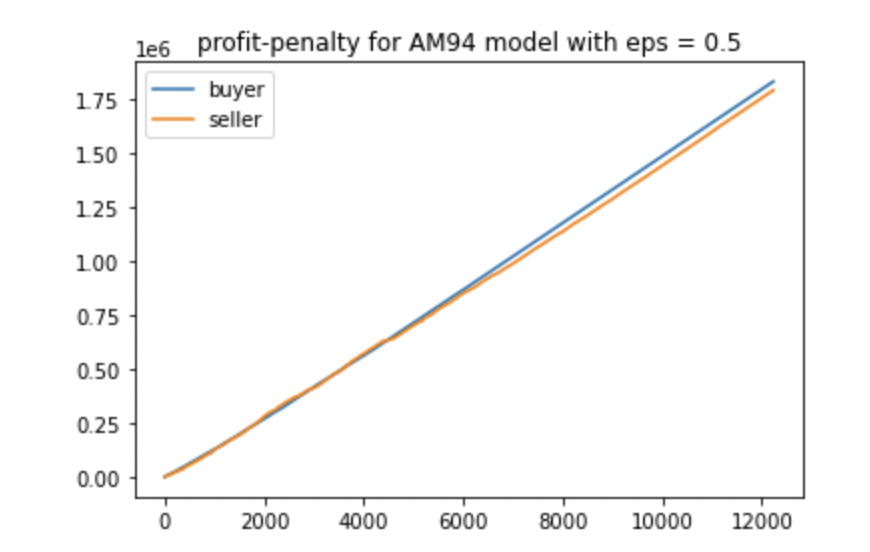
\includegraphics[width=0.9\textwidth]{21.PNG}
	\end{center}
	\caption{profit - penalty,no reward}
	\label{FIG.21}
\end{figure}	

If we consider only successful implementation situations, we can get other 3 pictures

\begin{figure}[H]
	\begin{center}
	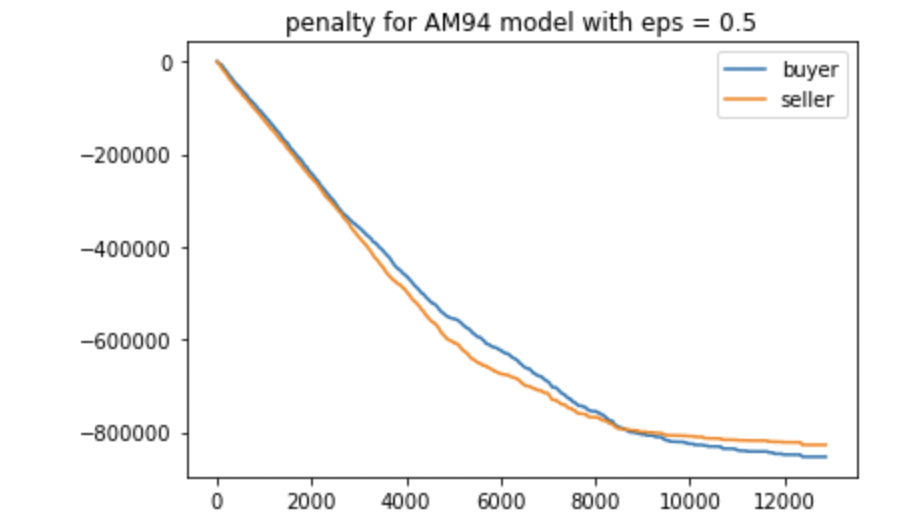
\includegraphics[width=0.9\textwidth]{22.PNG}
	\end{center}
	\caption{full penalty,no reward,implementation}
	\label{FIG.22}
\end{figure}

\begin{figure}[H]
	\begin{center}
	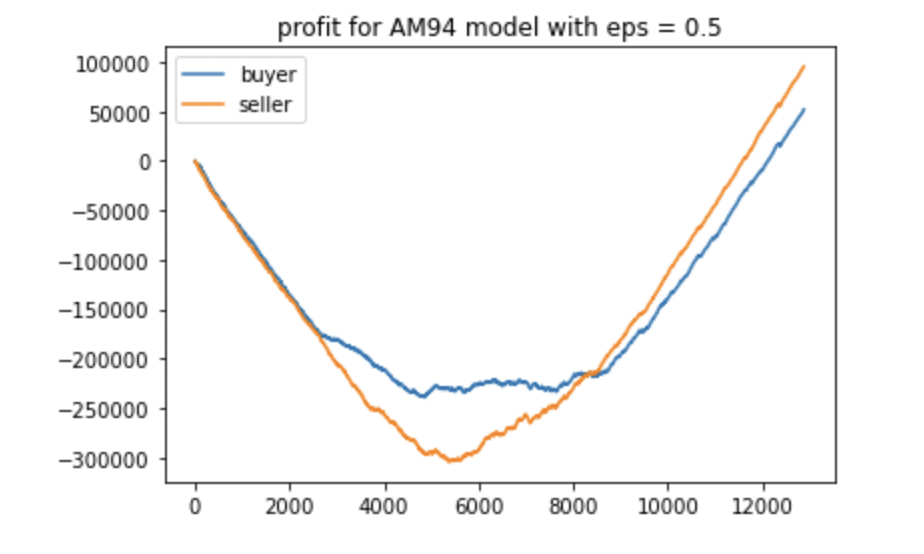
\includegraphics[width=0.9\textwidth]{23.PNG}
	\end{center}
	\caption{full profit,no reward,implementation}
	\label{FIG.23}
\end{figure}

\begin{figure}[H]
	\begin{center}
	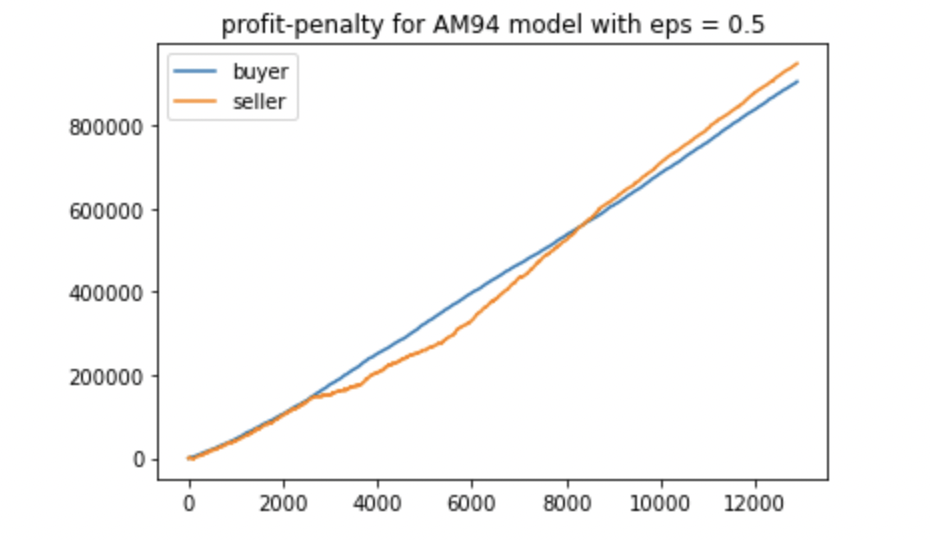
\includegraphics[width=0.9\textwidth]{24.PNG}
	\end{center}
	\caption{profit - penalty,no reward,implementation}
	\label{FIG.24}
\end{figure}

\subsubsection{AM94 with no reward on $\epsilon = 0.4$}

\begin{figure}[H]
	\begin{center}
	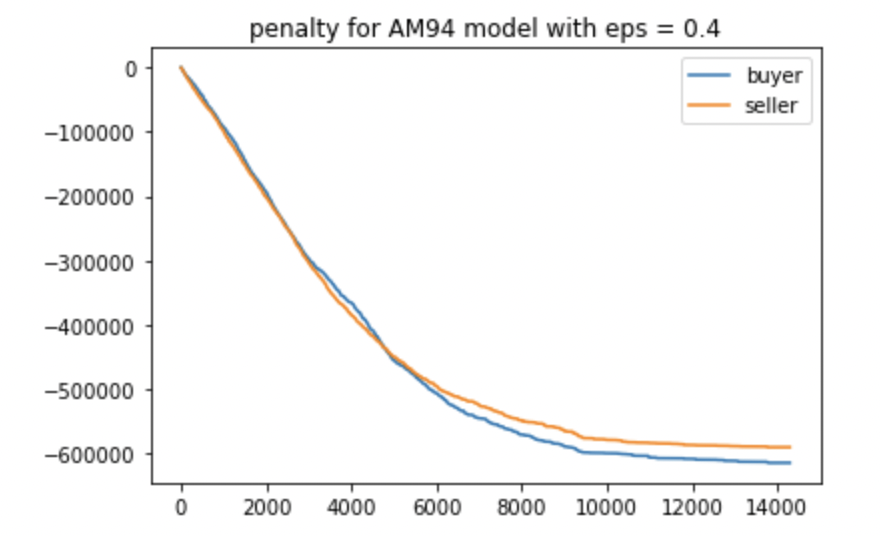
\includegraphics[width=0.9\textwidth]{25.PNG}
	\end{center}
	\caption{full penalty,no reward}
	\label{FIG.25}
\end{figure}

\begin{figure}[H]
	\begin{center}
	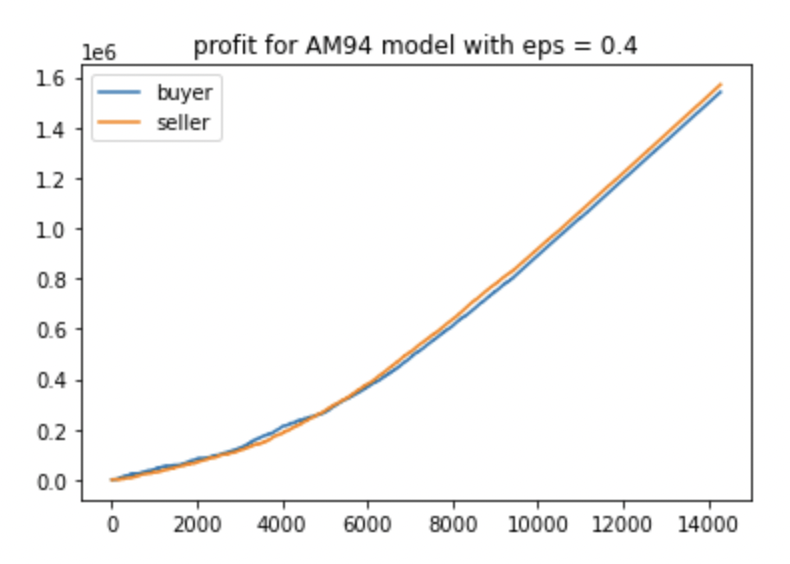
\includegraphics[width=0.9\textwidth]{26.PNG}
	\end{center}
	\caption{full profit,no reward}
	\label{FIG.26}
\end{figure}

\begin{figure}[H]
	\begin{center}
	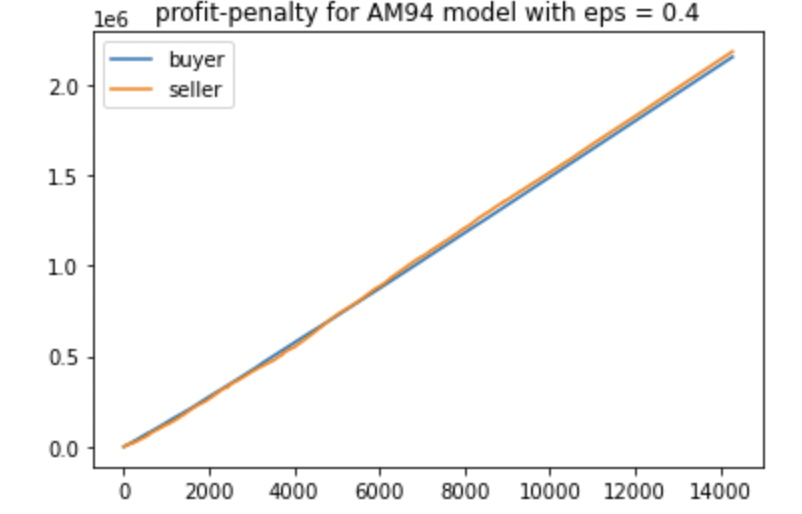
\includegraphics[width=0.9\textwidth]{27.PNG}
	\end{center}
	\caption{profit - penalty,no reward}
	\label{FIG.27}
\end{figure}	

If we consider only successful implementation situations, we can get other 3 pictures

\begin{figure}[H]
	\begin{center}
	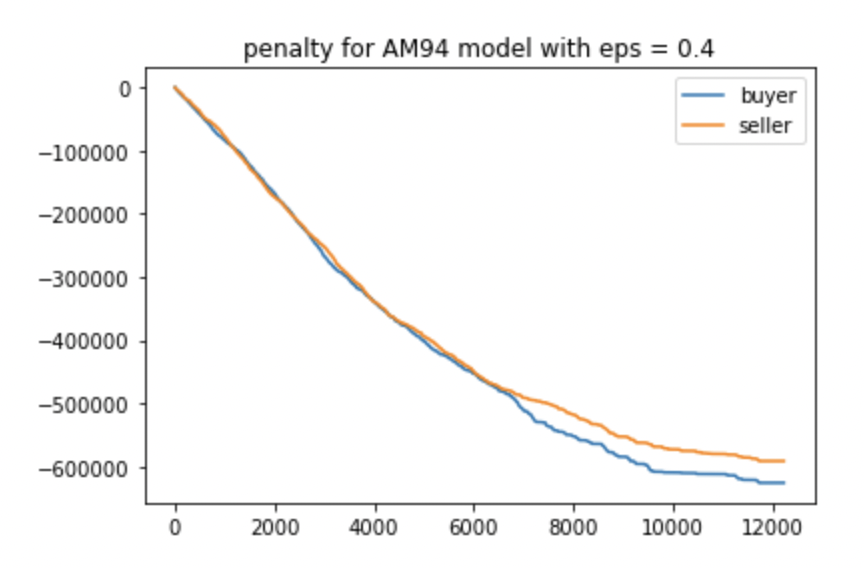
\includegraphics[width=0.9\textwidth]{28.PNG}
	\end{center}
	\caption{full penalty,,no rewardimplementation}
	\label{FIG.28}
\end{figure}

\begin{figure}[H]
	\begin{center}
	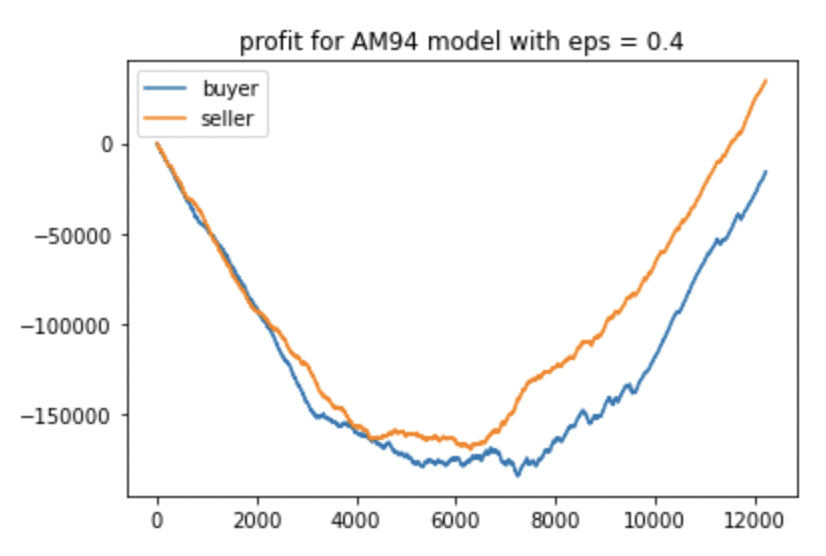
\includegraphics[width=0.9\textwidth]{29.PNG}
	\end{center}
	\caption{full profit,no reward,implementation}
	\label{FIG.29}
\end{figure}

\begin{figure}[H]
	\begin{center}
	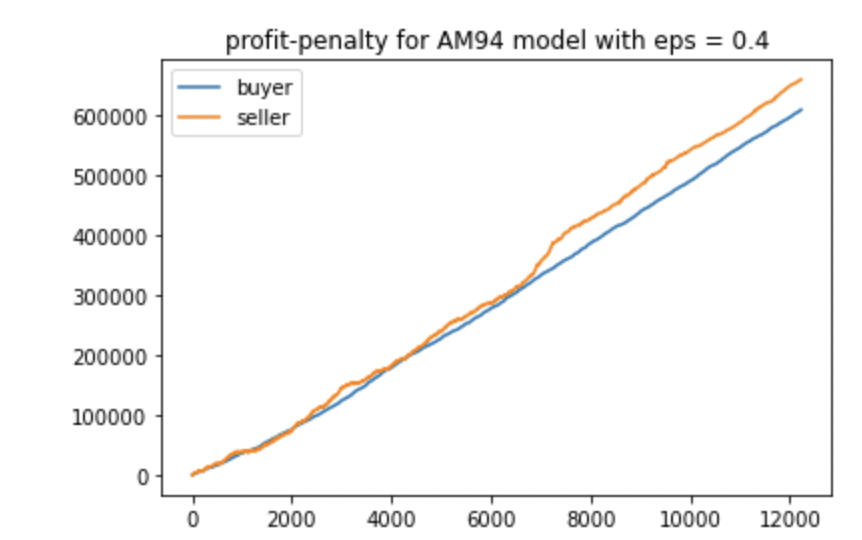
\includegraphics[width=0.9\textwidth]{30.PNG}
	\end{center}
	\caption{profit - penalty,no reward,implementation}
	\label{FIG.30}
\end{figure}


\subsubsection{AM94 with no reward on $\epsilon = 0.2$}
the turning point is around 0.22, so this result does not converge.

\begin{figure}[H]
	\begin{center}
	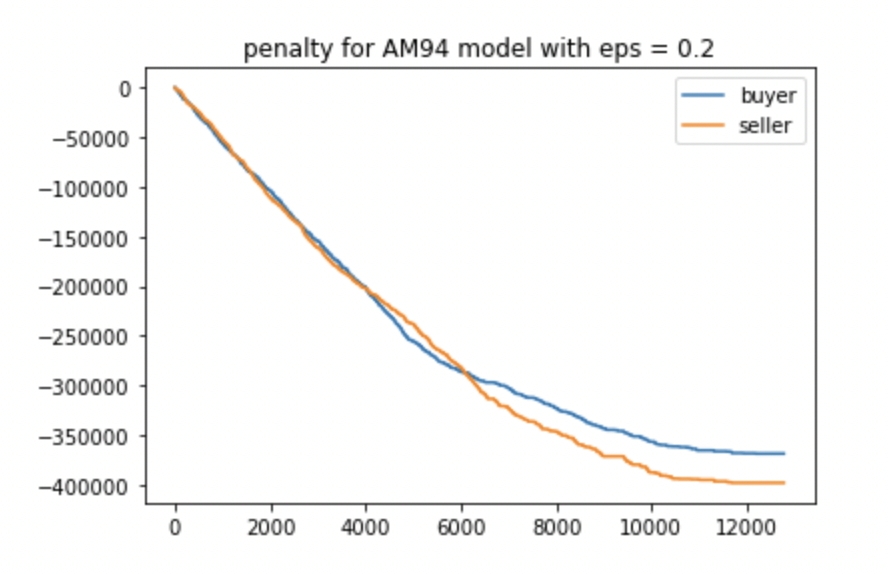
\includegraphics[width=0.9\textwidth]{31.PNG}
	\end{center}
	\caption{full penalty,no reward}
	\label{FIG.31}
\end{figure}

\begin{figure}[H]
	\begin{center}
	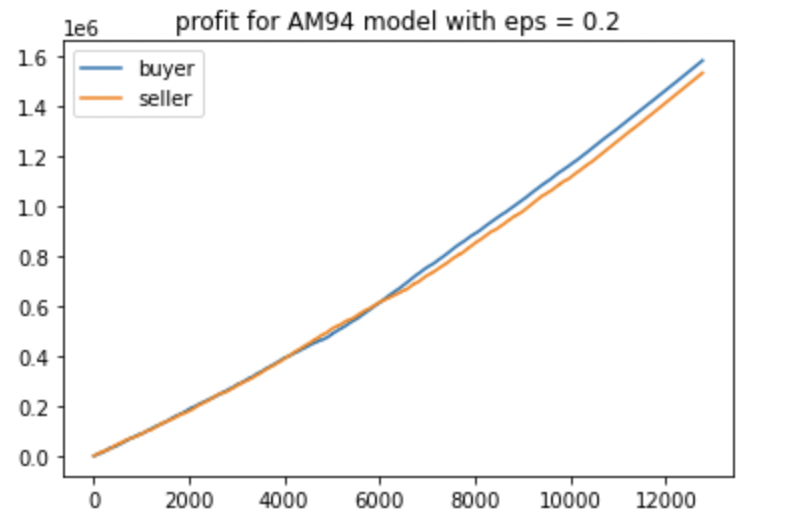
\includegraphics[width=0.9\textwidth]{32.PNG}
	\end{center}
	\caption{full profit,no reward}
	\label{FIG.32}
\end{figure}

\begin{figure}[H]
	\begin{center}
	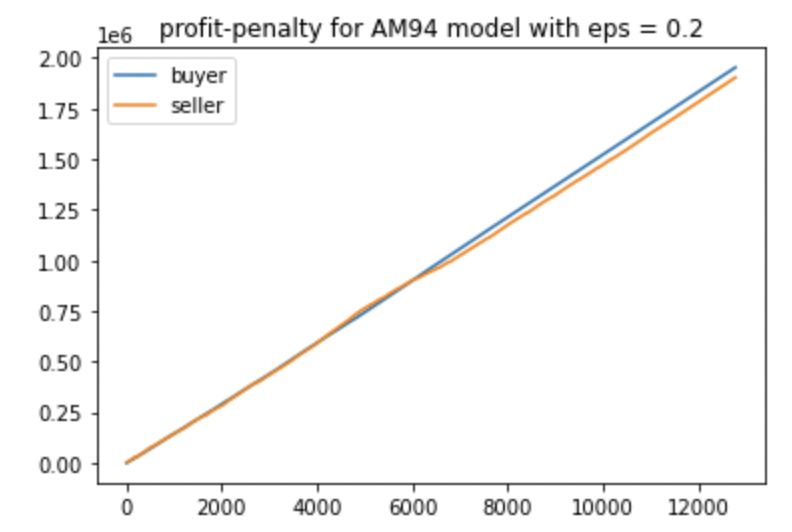
\includegraphics[width=0.9\textwidth]{33.PNG}
	\end{center}
	\caption{profit - penalty,no reward}
	\label{FIG.33}
\end{figure}	

If we consider only successful implementation situations, we can get other 3 pictures

\begin{figure}[H]
	\begin{center}
	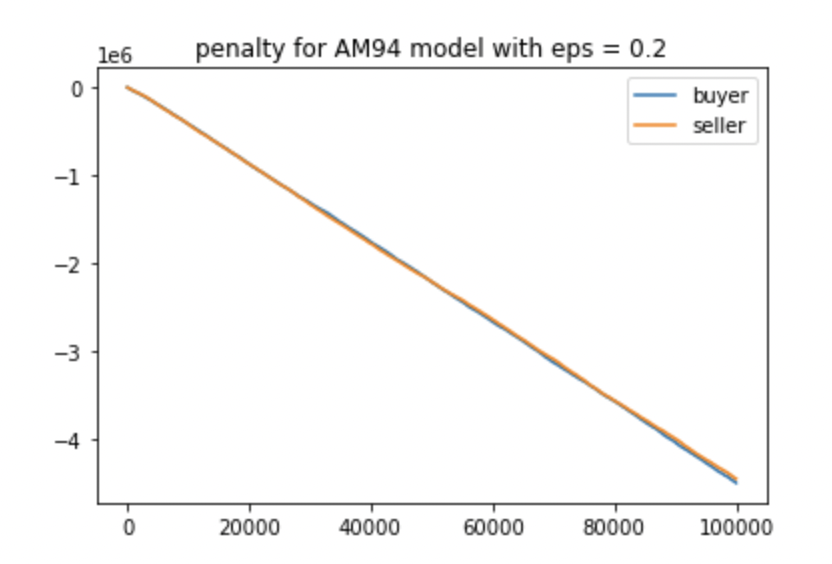
\includegraphics[width=0.9\textwidth]{34.PNG}
	\end{center}
	\caption{full penalty,no reward,implementation}
	\label{FIG.34}
\end{figure}

\begin{figure}[H]
	\begin{center}
	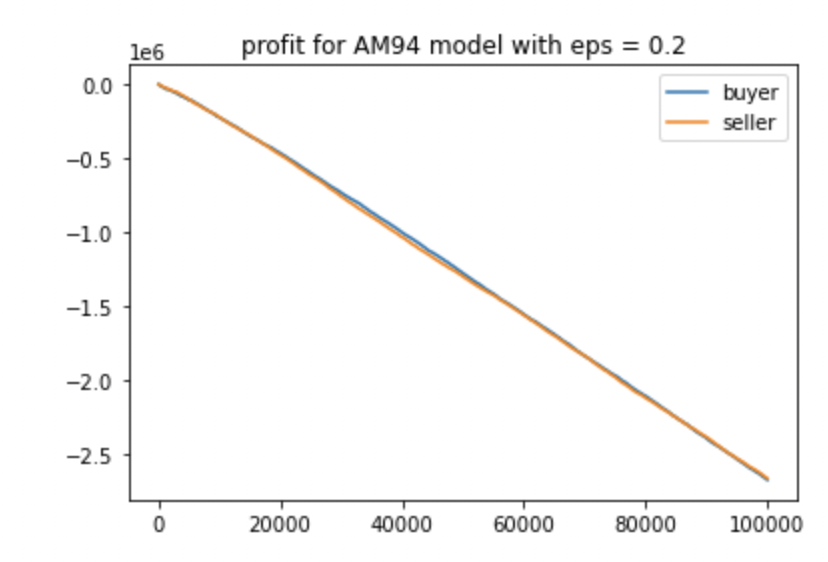
\includegraphics[width=0.9\textwidth]{35.PNG}
	\end{center}
	\caption{full profit,no reward,implementation}
	\label{FIG.35}
\end{figure}

\begin{figure}[H]
	\begin{center}
	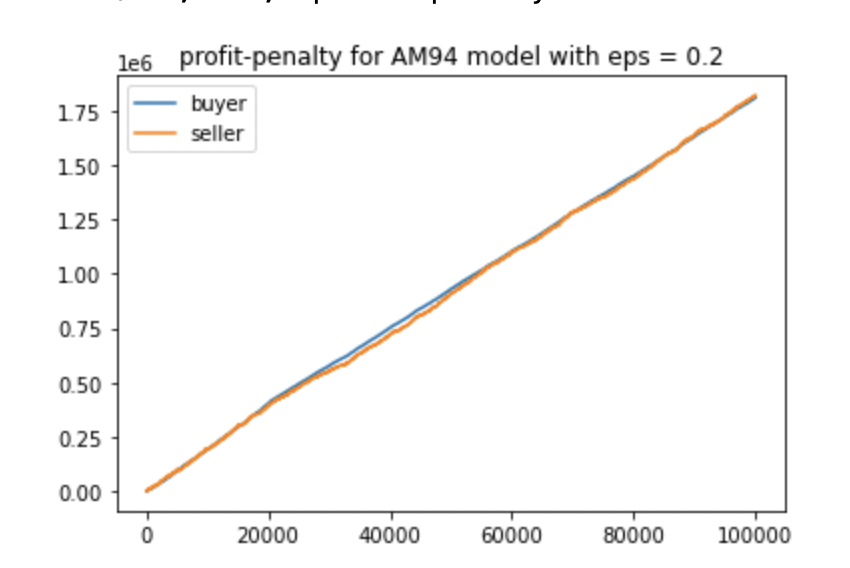
\includegraphics[width=0.9\textwidth]{36.PNG}
	\end{center}
	\caption{profit - penalty,no reward,implementation}
	\label{FIG.36}
\end{figure}


\subsection{AM model}
AM models can be compared with AM94 and SR models, all with no reward.
\subsubsection{AM on $\epsilon = 0.4$}

\begin{figure}[H]
	\begin{center}
	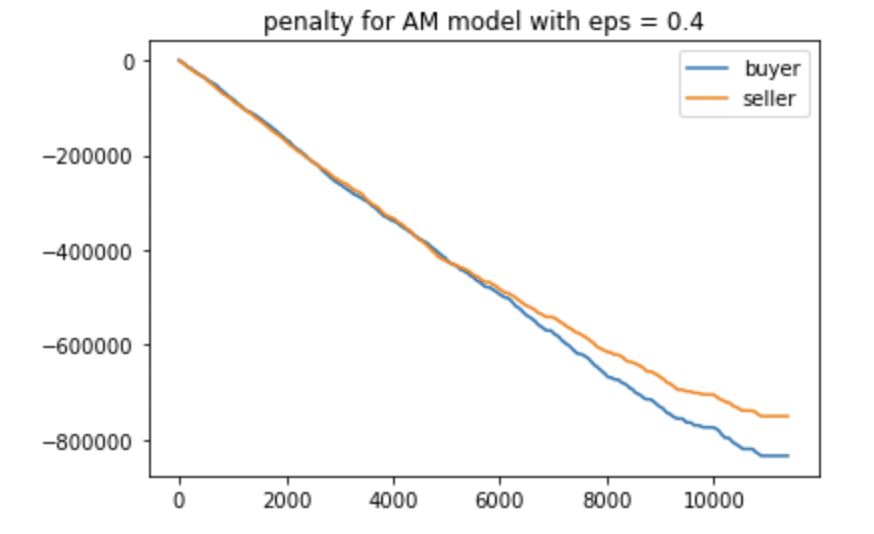
\includegraphics[width=0.9\textwidth]{37.PNG}
	\end{center}
	\caption{full penalty}
	\label{FIG.37}
\end{figure}

\begin{figure}[H]
	\begin{center}
	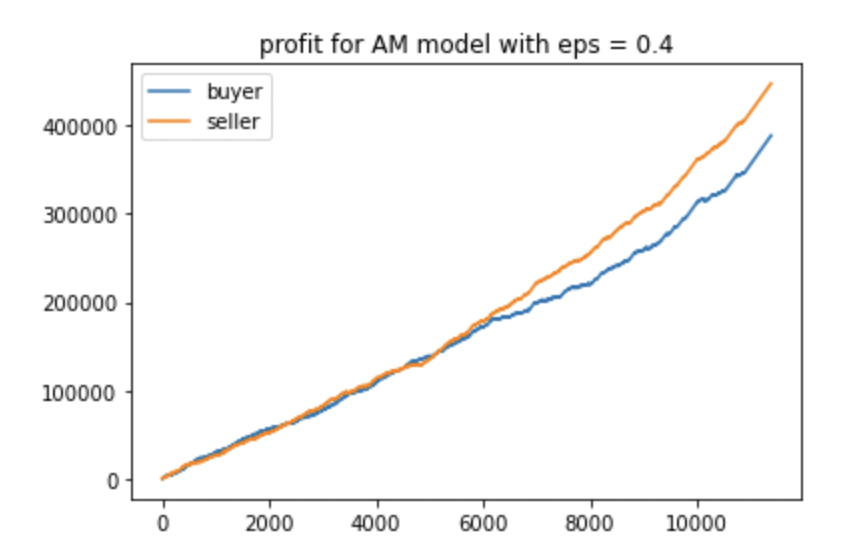
\includegraphics[width=0.9\textwidth]{38.PNG}
	\end{center}
	\caption{full profit}
	\label{FIG.38}
\end{figure}

\begin{figure}[H]
	\begin{center}
	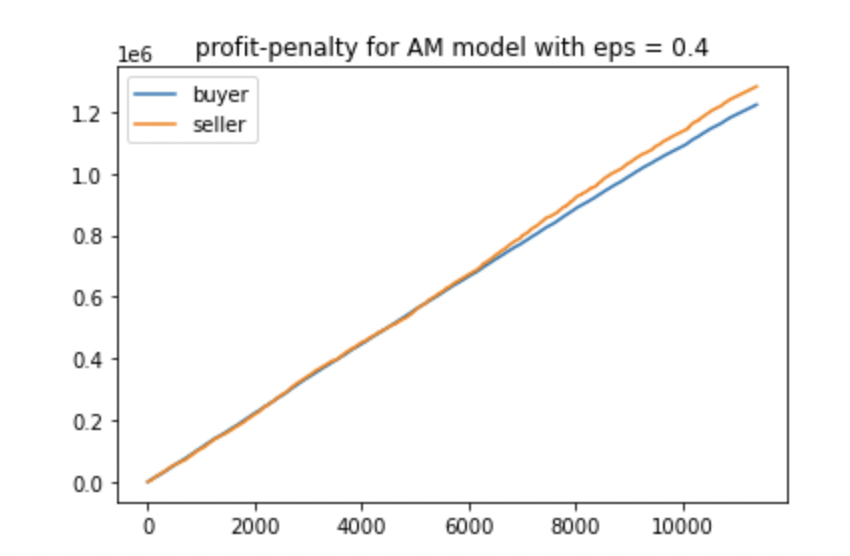
\includegraphics[width=0.9\textwidth]{39.PNG}
	\end{center}
	\caption{profit - penalty}
	\label{FIG.39}
\end{figure}	

If we consider only successful implementation situations, we can get other 3 pictures

\begin{figure}[H]
	\begin{center}
	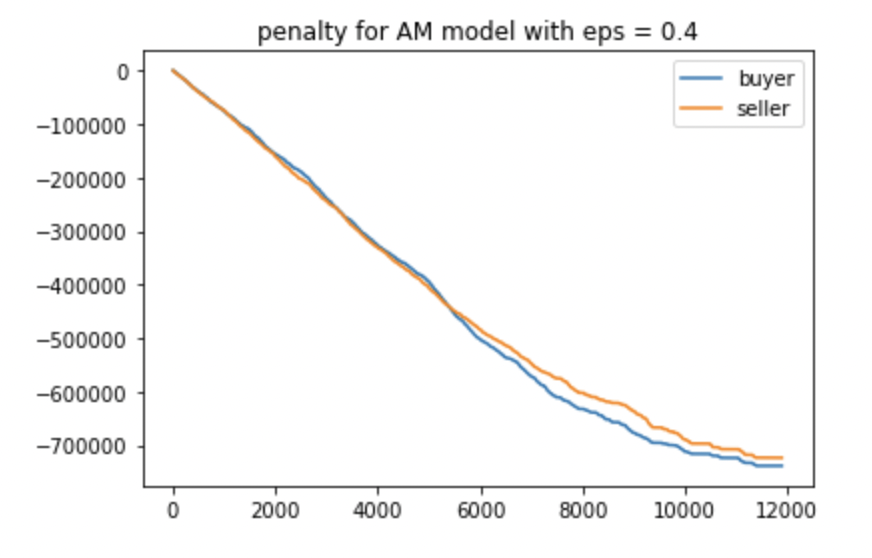
\includegraphics[width=0.9\textwidth]{40.PNG}
	\end{center}
	\caption{full penalty,implementation}
	\label{FIG.40}
\end{figure}

\begin{figure}[H]
	\begin{center}
	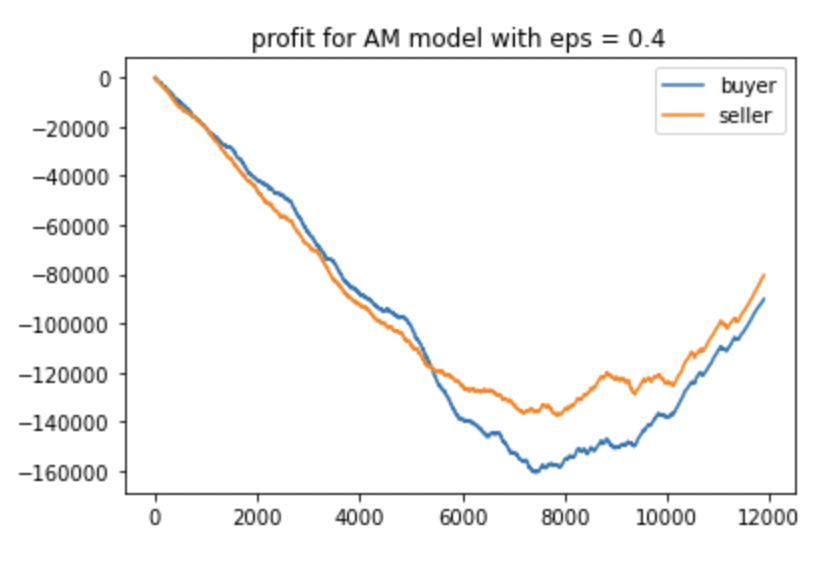
\includegraphics[width=0.9\textwidth]{41.PNG}
	\end{center}
	\caption{full profit,implementation}
	\label{FIG.41}
\end{figure}

\begin{figure}[H]
	\begin{center}
	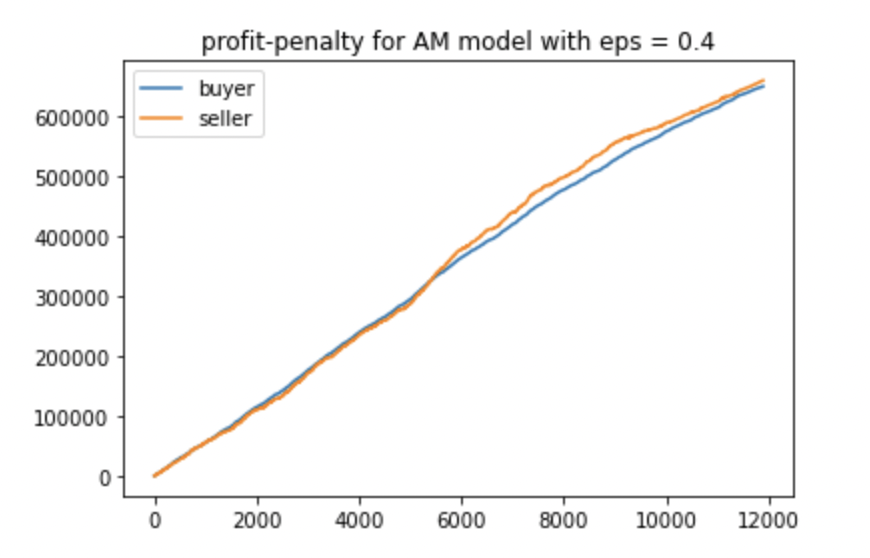
\includegraphics[width=0.9\textwidth]{42.PNG}
	\end{center}
	\caption{profit - penalty,implementation}
	\label{FIG.42}
\end{figure}

\subsubsection{AM94 with reward on $\epsilon = 0.3$}

\begin{figure}[H]
	\begin{center}
	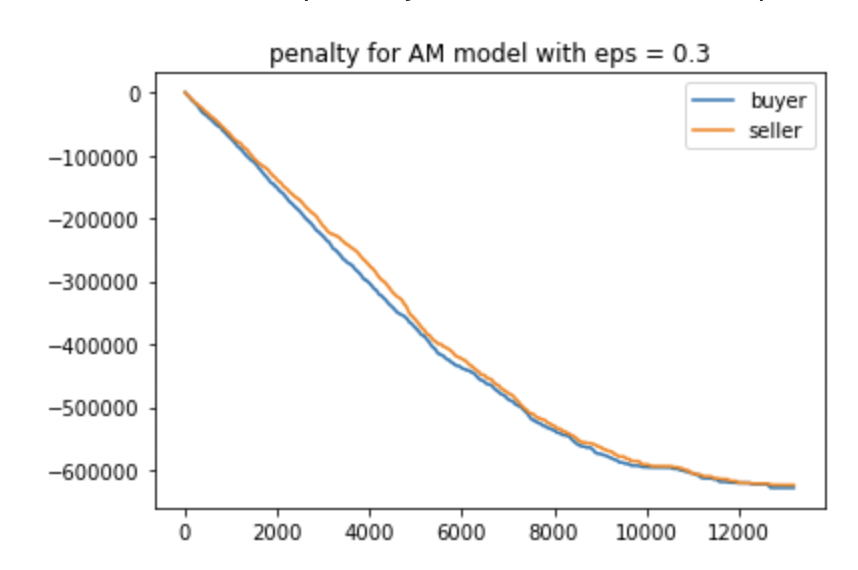
\includegraphics[width=0.9\textwidth]{43.PNG}
	\end{center}
	\caption{full penalty}
	\label{FIG.43}
\end{figure}

\begin{figure}[H]
	\begin{center}
	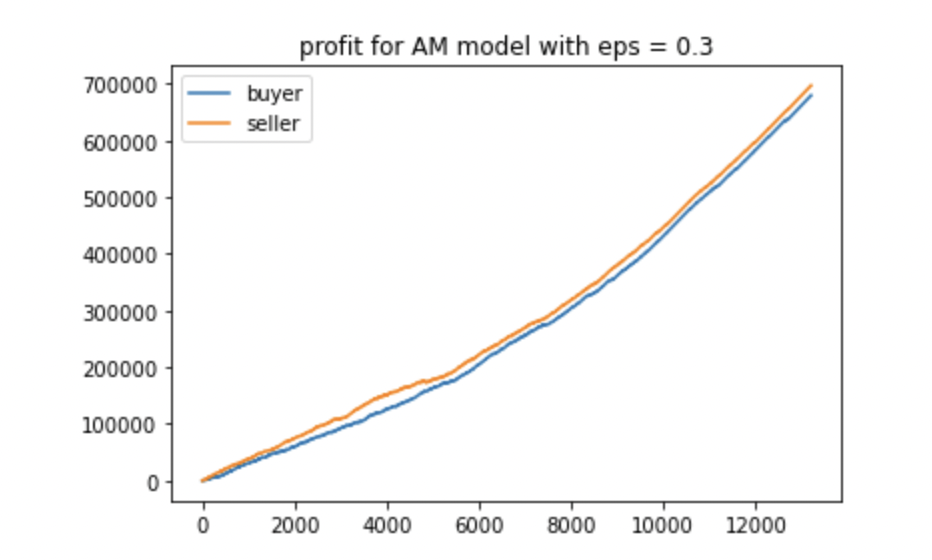
\includegraphics[width=0.9\textwidth]{44.PNG}
	\end{center}
	\caption{full profit}
	\label{FIG.44}
\end{figure}

\begin{figure}[H]
	\begin{center}
	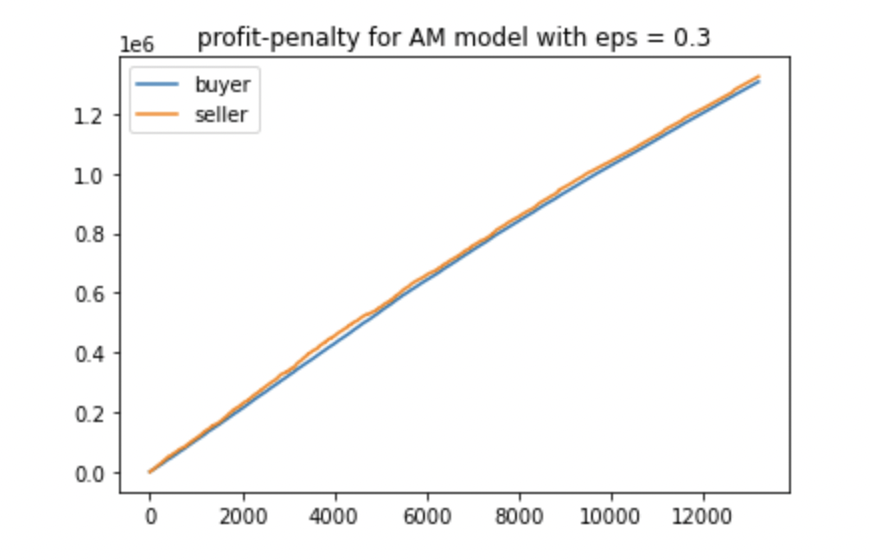
\includegraphics[width=0.9\textwidth]{45.PNG}
	\end{center}
	\caption{profit - penalty}
	\label{FIG.45}
\end{figure}	

If we consider only successful implementation situations, we can get other 3 pictures

\begin{figure}[H]
	\begin{center}
	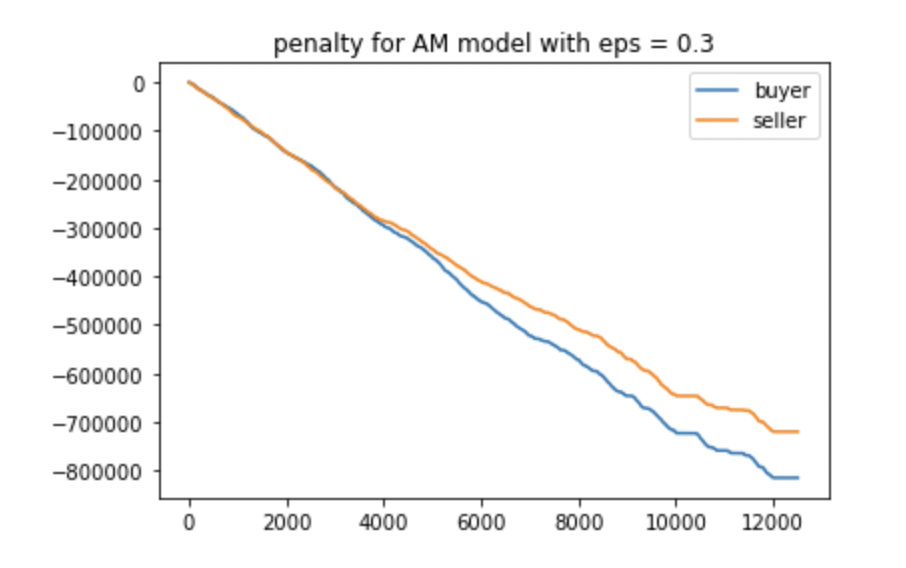
\includegraphics[width=0.9\textwidth]{46.PNG}
	\end{center}
	\caption{full penalty,implementation}
	\label{FIG.46}
\end{figure}

\begin{figure}[H]
	\begin{center}
	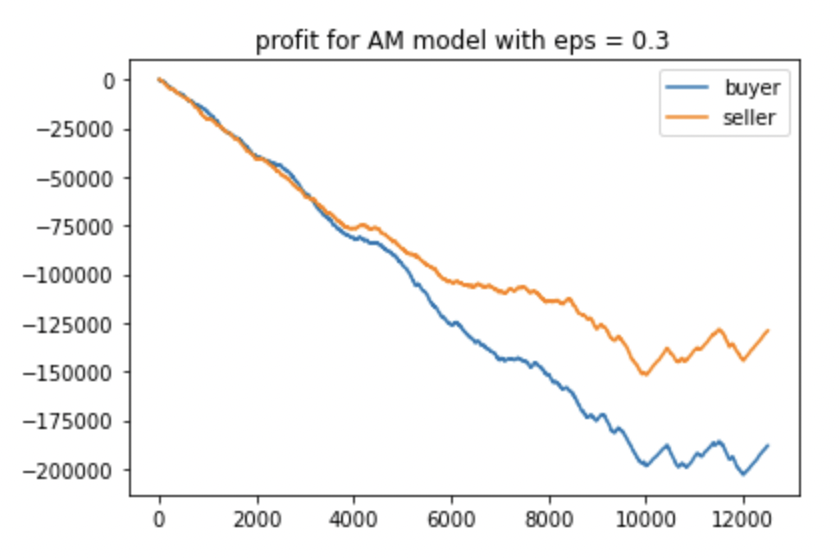
\includegraphics[width=0.9\textwidth]{47.PNG}
	\end{center}
	\caption{full profit,implementation}
	\label{FIG.47}
\end{figure}

\begin{figure}[H]
	\begin{center}
	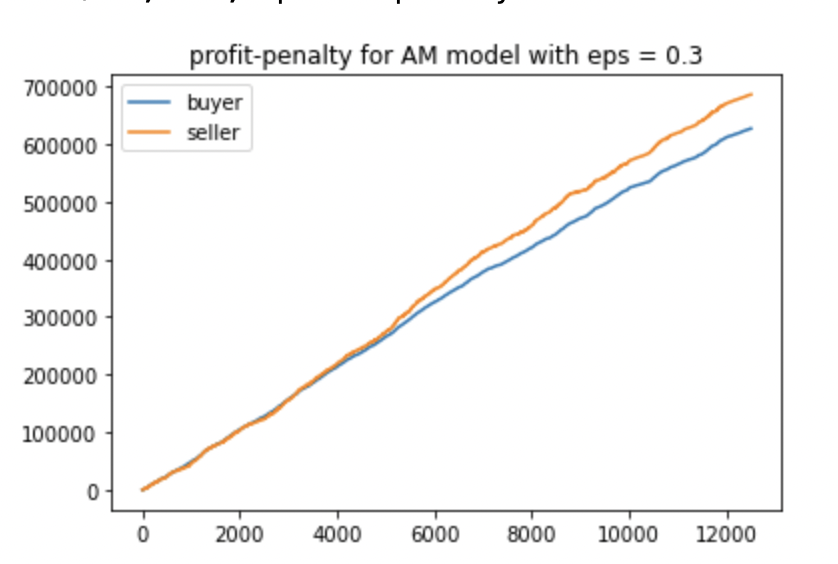
\includegraphics[width=0.9\textwidth]{48.PNG}
	\end{center}
	\caption{profit - penalty,implementation}
	\label{FIG.48}
\end{figure}


\subsubsection{AM94 with reward on $\epsilon = 0.2$}
the turning point is around 0.23, so this result does not converge.

\begin{figure}[H]
	\begin{center}
	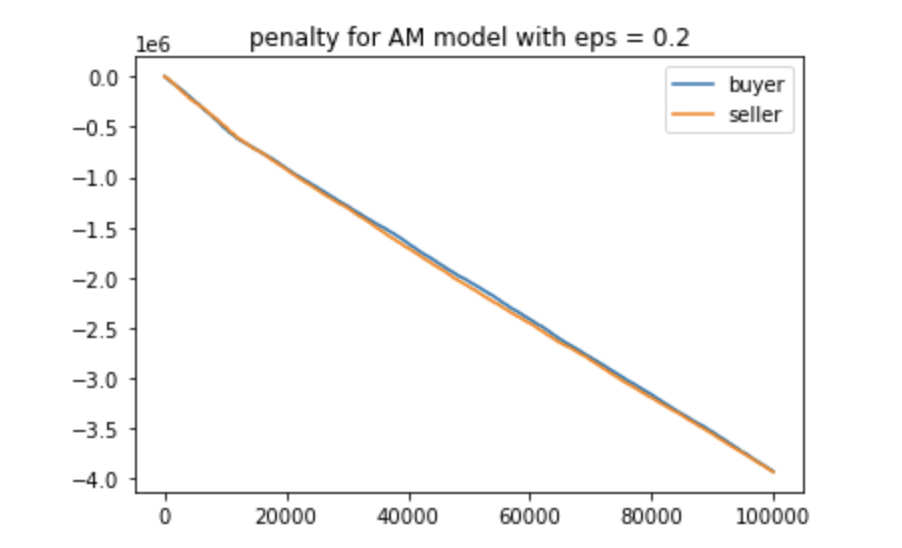
\includegraphics[width=0.9\textwidth]{49.PNG}
	\end{center}
	\caption{full penalty}
	\label{FIG.49}
\end{figure}

\begin{figure}[H]
	\begin{center}
	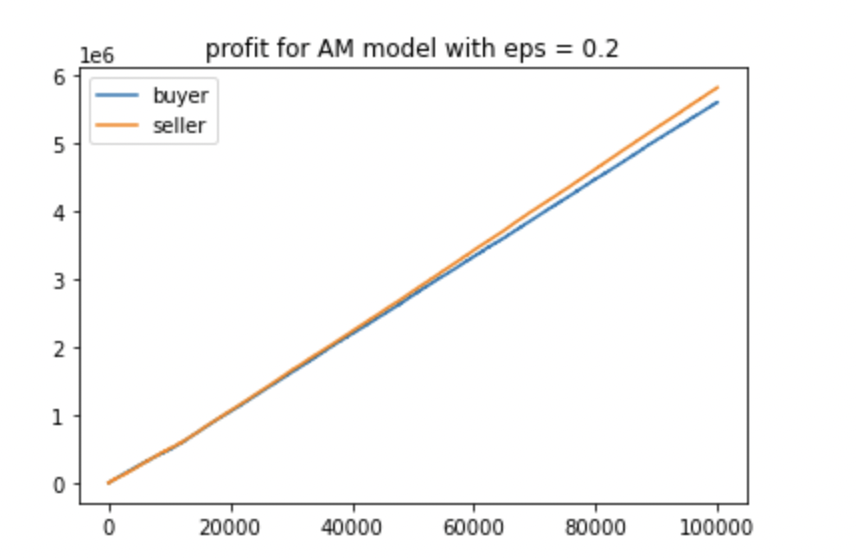
\includegraphics[width=0.9\textwidth]{50.PNG}
	\end{center}
	\caption{full profit}
	\label{FIG.50}
\end{figure}

\begin{figure}[H]
	\begin{center}
	\includegraphics[width=0.9\textwidth]{51.PNG}
	\end{center}
	\caption{profit - penalty}
	\label{FIG.51}
\end{figure}	

If we consider only successful implementation situations, we can get other 3 pictures

\begin{figure}[H]
	\begin{center}
	\includegraphics[width=0.9\textwidth]{52.PNG}
	\end{center}
	\caption{full penalty,implementation}
	\label{FIG.52}
\end{figure}

\begin{figure}[H]
	\begin{center}
	\includegraphics[width=0.9\textwidth]{53.PNG}
	\end{center}
	\caption{full profit,implementation}
	\label{FIG.53}
\end{figure}

\begin{figure}[H]
	\begin{center}
	\includegraphics[width=0.9\textwidth]{54.PNG}
	\end{center}
	\caption{profit - penalty,implementation}
	\label{FIG.54}
\end{figure}

\subsection{SR model}
SR models have no $\epsilon$.

\subsubsection{SR model}

\begin{figure}[H]
	\begin{center}
	\includegraphics[width=0.9\textwidth]{55.PNG}
	\end{center}
	\caption{full penalty}
	\label{FIG.55}
\end{figure}

\begin{figure}[H]
	\begin{center}
	\includegraphics[width=0.9\textwidth]{56.PNG}
	\end{center}
	\caption{full profit}
	\label{FIG.56}
\end{figure}

\begin{figure}[H]
	\begin{center}
	\includegraphics[width=0.9\textwidth]{57.PNG}
	\end{center}
	\caption{profit - penalty}
	\label{FIG.57}
\end{figure}	


\section{Relearning Study of AM Models with Different $\epsilon$}

If we relax the $\epsilon$ of the AM model, players need to undergo relearning 
to achieve a converged state. Starting from the converged state, different $\epsilon$
values lead to varying outcomes in terms of re-convergence. As shown in the figure below.

\begin{figure}[H]
	\begin{center}
	\includegraphics[width=0.9\textwidth]{58.PNG}
	\end{center}
	\caption{relearning study for AM with different $\epsilon$}
	\label{FIG.58}
\end{figure}

In the picture different lines stand for different $\epsilon$, the lower the lines
the smaller the $\epsilon$

the conclusion that can be drawn is that relearning states that do not converge, 
regardless of their lack of convergence, still do not converge, 
as long as they are below the turning point.

If we retrain the SR model and transition from a converged state to a non-converged 
state, each time we can return to the converged state, as shown in the figure.

\begin{figure}[H]
	\begin{center}
	\includegraphics[width=0.9\textwidth]{59.PNG}
	\end{center}
	\caption{relearning study for SR}
	\label{FIG.59}
\end{figure}

In the picture we choose different state, we can see that all state will go to convergence
state


\section{Future work}
\begin{itemize}
  \item [0)]
  	Attempt to identify a parameter set applicable to all states, rather than 
	restricting it solely to states (2,2) and states (2,1). Execute the parameter 
	loop across all scenarios and then contrast the outcomes with those of 
	states (2,2) and states (2,1).
  \item [1)]
  	Conduct an $\epsilon$ cycle, experimenting with a broader range of $\epsilon$
	values across all models. The goal is to pinpoint the precise turning point for 
	each model.
\end{itemize}

\end{document} 